In this section, we discuss the relationship of the various
\textsc{EviL} logics developed in this section.  
Using the observed relationships, as well as our 
previously derived small model properties,  
we shall present some basic known complexity 
results for satisfiability in these various logics.

We shall first prove the following lemma:

\begin{lemma}
\textsc{EviL}, \textsc{EviL}$^\BM$ and \textsc{EviL}$^\BP$ with a single agent are all conservative extensions of the basic modal logic with just axiom $K$.  That is, if $\nvdash_K \phi$ then $\nvdash_{\textup{\textsc{EviL}}} \phi$ and similarly for the fragments \textsc{EviL}$^\BM$ and \textsc{EviL}$^\BP$.

\textsc{EviL} with $m > n$ agents is a conservative extension of \textsc{EviL} with $n$ agents, and likewise for the fragments \textsc{EviL}$^\BM$ and \textsc{EviL}$^\BP$ 
\end{lemma}
\begin{proof}
Assume that $\nvdash_K \phi$, then we know from modal logic that there's a finite Kripke Structure $\mathbb{M} := \langle W, V, R\rangle$ such and a world $w \in W$ such that $\mathbb{M},w \nvdash \phi$.  Now extend $\mathbb{M}$ to $\mathbb{M}' := \langle W, V, P, R_\Nec, R_\BB, R_\BBI \rangle$ where
\begin{bul}
	\item $P := \{(v,v)\ |\ v R v\}$
	\item $R_\BB := R_\BBI := \{(w,w)\ |\ w \in W\}$
\end{bul}
This model is trivially completely \textsc{EviL}. Moreover we know that $\mathbb{M}$ is an elementary submodel of $\mathbb{M}'$, so $\mathbb{M}', w\nvdash \phi$.  Hence by the Lemma \ref{translation-lemma} we have a model $\mathfrak{M}$ and $(a,A) \in \mathfrak{M}$ such that $\mathfrak{M},(a,A) \nmodels \phi$; so by soundness for \textsc{EviL} we have the desired result.

Similarly, if we $\nvdash_{\textup{\textsc{EviL}}_\mathcal{A}} \phi$ then by completeness can find a witnessing $\mathfrak{M}$ and $(a,A) \in \mathfrak{M}$ such that $\mathfrak{M},(a,A) \nmodels \phi$.  But then we can embed $\mathfrak{M}$ into $\mathfrak{M}'$ for agents $\mathcal{B} \supseteq \mathcal{A}$ where $\mathfrak{M}' := \{(a,A') \ |\ (a,A) \in \mathfrak{M}\}$ and
$$ A'_X := \begin{cases} A_X & X \in\mathcal{A} \\ \varnothing & X \nin \mathcal{A}\end{cases} $$
\end{proof}

By similar arguments, \textsc{EviL} is a conservative extension of \textsc{EviL}$^\BM$ and \textsc{EviL}$^\BP$, and that all three of these are conservative extensions of $K$.  This is summerized in the Fig. \ref{conservative-extensions}.

\begin{figure}[ht]
\begin{center}
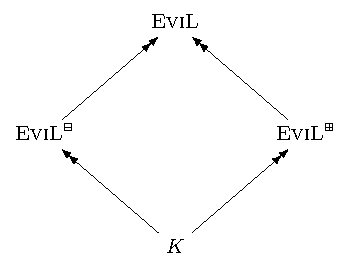
\includegraphics[]{logics/evils.pdf}
\end{center}
\caption{\textsc{EviL} conservative extensions of $K$}
\label{conservative-extensions}
\end{figure}

\begin{lemma}
	\textsc{EviL} is \textsf{PSPACE} hard 
\end{lemma}
\begin{proof}
This follows trivially from the fact that \textsc{EviL} is a conservative extension of basic modal logic, and the decision problem for basic modal logic is \textsf{PSPACE} complete.
\end{proof}

%%% Local Variables: 
%%% mode: latex
%%% TeX-master: "evil_philosophy"
%%% End: 
